\documentclass[a4paper, oneside, final]{scrartcl}

\usepackage{scrlayer-scrpage}
\usepackage{titlesec}
\usepackage{anysize}
\usepackage{marvosym}
\usepackage{tabularx,colortbl}
\usepackage{ebgaramond}
\usepackage{microtype}
\usepackage{hyperref}
\usepackage{graphicx}
\usepackage{amsmath}

\titleformat{\section}{\large\scshape\raggedright}{}{0em}{}[\titlerule]

\pagestyle{scrheadings}

\addtolength{\voffset}{-0.5in}
\addtolength{\textheight}{3cm}

\newcommand{\gray}{\rowcolor[gray]{.90}}

\renewcommand{\headfont}{\normalfont\rmfamily}

\marginsize{2cm}{2cm}{2cm}{2cm}
\setlength{\parindent}{0cm}

\begin{document}

\thispagestyle{empty}

\begin{center}
    %\newcommand{\HRule}{\rule{\linewidth}{0.5mm}}
    \begin{minipage}{0.29\textwidth} 
        \center{
\includegraphics[scale = 0.06]{images/logo_unam.png}}
    \end{minipage}
    \begin{minipage}{0.40\textwidth} 
    \center{\textsc{\LARGE Universidad Nacional \\[5mm] Autónoma de México}}\\
    \end{minipage}
    \begin{minipage}{0.29\textwidth}
        \center{
\includegraphics[scale =0.18]{images/logo_ciencias.png}}
    \end{minipage}
    \vspace{5mm}					
    
    \textsc{\noindent \LARGE Facultad de Ciencias}\\[20mm]
    
    \textsc{\LARGE   Ingeniería de Software \\[5mm]
                    \LARGE 2024-2}      \\[20mm]
    
    \textsc{\textbf{\huge   Análisis de requerimientos}}\\[5mm]
    \textsc{\LARGE  Pizarra colaborativa para computólogos}\\[20mm]

    \LARGE
    \textsc{Equipo I}\\[5mm]
    \Large 
    \textsc{Diego Sebastián Sánchez Correa}\\[2mm]
    \textsc{Mauro Emiliano Chávez Zamora}\\[2mm]
    \textsc{Ulises Josué Anaya Pérez}\\[2mm]
    \textsc{Daniel Linares Gil} \\[2mm]
    \textsc{Karyme Ivette Azpeitia García}
    \\[20mm]

    \large Creado: 15/02/2024\\[2mm]
    \large Última actualización: 20/02/2024\\
    
\end{center}	
\newpage  


\section{--Resumen--}

Pretendemos desarrollar una herramienta útil que satisfaga las
necesidades esenciales para el desarrollo de proyectos relacionados con las ciencias de la computación. De manera que se facilite colaborar en un mismo documento que integre múltiples herramientas para graficar funciones, escribir texto plano, dibujar con algo de sultura, analizar problemas matemáticos a través de la facilidad para escribir ecuaciones y que al mismo tiempo permita agruparlas por practicidad.\\

La idea de un editor de texto con \textit{syntax highlighting} es común dentro
del ámbito de desarrollo de software, sin embargo, se carece de herramientas de
planeación colaborativa donde las ideas se puedan aterrizar de manera general o
con detalles tan específicos como los usuarios lo deseen. De manera que nuestra propuesta busca cumplir esa función aunque sea a través de unas cuanta funcionalidades básicas. Esta aplicación tiene como fin la creación de un ambiente colaborativo y cuya
esencia sirva como punto de partida para la elaboración de decisiones de diseño
a partir de diagramas, control de versiones, edición con dibujo vectorizado y
soporte para \LaTeX.\\

Si bien existen múltiples herramientas para simular pizarrones, de las cuales muchas tomaron relevancia durante la pandemia del 2020, al forzarse las actividades en línea, no ha sido especialmente sencillo para personas en licenciatura expresar sus complejas o específicas notaciones con facilidad, no sólo por la falta de habilidad al usar equipos de cómputo sino porque la forma de hacerlo brindada por los desarrolladores no ha sido la más eficaz. Si bien no es nuestra labor capacitar a las personas en el uso de sus equipos, sí podemos desarrollar herramientas que faciliten las labores académicas o laborales de las personas en ciencias de la computación.
Tenemos como ejemplos algunas otras herramientas de pizarra colaborativa: \href{https://miro.com/}{Miro}, \href{https://www.mural.co/}{Mural}, \href{ https://www.microsoft.com/en-us/microsoft-365/microsoft-whiteboard/digital-whiteboard-app}{Microsoft Whiteboard},\href{https://www.figma.com/figjam/}{Figjam} y \href{https://jamboard.google.com}{Jamboard}.

\section{--Ejemplos de uso:--}

\textbf{Entrevista de programación:} Alice se encuentra entrevistando candidatos para unirse a su equipo como
    desarrolladores de software, la mayoría de entrevistas en su compañía se hacen a través de videollamadas ya que el trabajo es a distancia. Alice decide utilizar nuestra pizarra colaborativa porque permite bloques de código,
    dibujar de manera libre y escribir diagramas para explicar la solución. Durante la entrevista, el candidato escribe
    su solución en el bloque de código y además puede utilizar las funcionalidades de diagramado y dibujo libre para explicar su solución a Alice.

\textbf{Reunión de retrospectiva:} Alice se prepara para la reunión de retrospectiva de su equipo de desarrollo luego de un sprint. Alice crea una nueva pizarra, y la divide en tres columnas:
una sobre qué fue bien, una sobre qué no salió bien y la tercera sobre qué pueden mejorar.

Cuando Alice haya terminado de preparar la pizarra para la reunión, crea un enlace para compartir la pizarra y lo comparte con los miembros de su equipo. Durante la reunión, los miembros del equipos colaboran añadiendo notas en cada columna, dan sus propias impresiones sobre el desarrollo del proyecto y la conversación se mantiene tan dinámica como la pizarra. También pueden incluir enlaces a los tickets de Jira correspondientes en las notas. Una vez terminan de añadir notas, los miembros del equipo discuten sobre estas.
\clearpage

\section{--Requerimientos--}

\section{1.-Integración de Diagramas y Codificación}


  Deseamos proveer un ambiente donde los desarrolladores pueden crear diagramas lo cuales puedan complementar en aplicaciones concretas de
  código en el mismo espacio, facilitando con ello la visualización y la
  implementación simultánea de ideas. Existen conceptos matemáticos básicos que requieren esquemas para expresarse de mejor manera, como la elaboración de autómatas de estado finito, hasta
  la integración de diagramas de flujo permitirán que las personas usuarias puedan ser
  capaces de definir las bases, algoritmos y diseño de un proyecto cuya esencia
  tenga una naturaleza colaborativa.\\

En el caso de la planificación de proyectos de software podría ser muy ilustrativo incluir código que esté relacionado con diagramas de flujo que representen el problema a resolver o rutinas necesarias para su finalización, además de ilustrar secciones breves del programa. Proyectamos que también incluya un editor de notas, ya que organizar en diagramas facilita que se utilice como una
    aplicación para tomar notas de forma cómoda, éstas notas también deberían poder hacerse de manera suplementaria al contenido de la pizarra. Además, la incorporación de
    formatos para código, puede brindar apoyo para estudiantes
    de carreras que estén relacionadas con el desarrollo de software. De forma avanzada podría permitir código colaborativo, de manera que sea sencillo conectarse a distancia para programar desde los horarios que permitan a las personas que usen la aplicación.

\noindent
\section{ 2.- Colaboración Concurrente} %daniel

 El objetivo de la pizarra es fomentar la colaboración y el intercambio de ideas entre usuarios, para lo cual es fundamental que la pizarra permita la colaboración en tiempo real entre los usuarios. Del lado de nuestro equipo queda la tarea de permitir que múltiples usuarios trabajen de manera simultanea en la pizarra. Una funcionalidad que consideramos vital con para el objetivo sería tener la posibilidad de compartir una pizarra a través de un enlace, se generará un enlace único para compartir la pizarra con otros usuarios de manera sencilla, a través de la simple acción de copiar y pegar el vínculo generado.\\


Para mejor privacidad de las personas que usen la plataforma, sólo aquellas personas autenticadas (o con cuenta) dentro de la plataforma podrán acceder a través de los enlaces para compartir una pizarra. Si una persona que no se encuentra autenticada o que no posee una cuenta intenta acceder a un enlace, será re-dirigida al flujo de autenticación/registro y luego a la pizarra. La persona debe poder elegir el nivel de acceso que se concede a los usuarios con el enlace; sólo lectura o lectura con permisos de edición. La primera permite a los usuarios con el enlace ver la pizarra, pero no realizar cambios, la segunda permite a los usuarios con el enlace ver y además editar la pizarra. La persona debe poder revocar el acceso a la pizarra en cualquier momento.\\

Una buena coordinación depende de que las personas puedan tener un referente preciso del estado actual de la pizarra, así que los usuarios que se encuentren trabajando en una pizarra deben poder visualizar en tiempo real las modificaciones realizadas a la pizarra por otros usuarios. Tendremos disponibles en la aplicación iconos indicadores de presencia de un usuario para una pizarra, deben poder ver ser visibles en la barra superior los avatares de los usuarios que están conectados a la pizarra. Además se podrá observar el cursor en tiempo real para indicar en qué sección están trabajando.


\noindent
\section{3.- Guardado Automático y Control de Versiones} %kary

  El guardado automático protege contra la pérdida de datos en caso de fallos del sistema, errores del usuario o eventos inesperados y el control de versiones permitiría que los usuarios trabajar juntos en la misma pizarra virtual de forma eficiente; a través de rastrear los cambios, deshacer errores y restaurar versiones anteriores. Como equipo buscamos garantizar la seguridad de los datos, facilitar la colaboración y mejorar la productividad de los usuarios.\\

  
 En cuanto a la frecuencia de los cambios proyectamos una opción de guardado automático de frecuencia configurable entre cada 5, 10 o 15 minutos. En caso de que no esté dentro de los alcances de tiempo existirá un botón que las personas apretarán para que vaya registrando sus cambios siempre que las personas lo tengan, similar al icono de guardado en una aplicación de computadora convencional.\\
    
Los archivos guardados automáticamente se deben almacenar en un servidor seguro y accesible para el usuario, como una nube privada(por ejemplo, Google Drive, Dropbox), servidor local o almacenamiento propio de la aplicación. La persona debe recibir una notificación cada vez que se guarde automáticamente su trabajo. La notificación indicará: fecha y hora del guardado, así como ubicación del archivo guardado. A través de éstas la persona debe poder restaurar una versión anterior de la pizarra en cualquier momento y revisar el historial de versiones.\\

El historial de versiones anteriores debe mostrarse como una lista de versiones con fecha y hora, donde haya miniaturas de cada versión. De la cual se podrá seleccionar una versión de la pizarra de la lista de versiones, usar un atajo de teclado o botón de "Restaurar" en la barra de herramientas. La persona debe poder deshacer los últimos cambios realizados en la pizarra con un botón de "Deshacer" en la barra de herramientas o con un atajo de teclado.
    




\section{4.- Pizarra expansible} %mauro

 Al momento de trabajar en múltiples pizarras puede ser sencillo que se pierda información relevante durante los cambios de pizarra, si bien lo ideal sería que los temas pudieran agruparse en una pizarra en específico cada uno. Hay temas que requerirán más espacio debido a los múltiples elementos que pueden componer una tarea/tema con muchos componentes o pasos.\\

  Nosotros en la aplicación buscamos ofrecer más espacio en pizarra conforme los usuarios añadan elementos en pantalla (notas, inserciones de Latex, etc). Como característica adicional, la aplicación emitirá un aviso cuando una pizarra sea demasiado grande, para sugerir al usuario segmentar el tema en múltiples pizarras. El usuario puede solicitar espacio a demanda conforme elige qué sitios del proyecto conviene ampliar en una determinada dirección, de manera que las personas pueda elegir qué tanto van a requerir de la aplicación.


\noindent
\section{5.-Registro de Usuarios} %ulises

    Para que los usuarios puedan guardar el progreso de su trabajo realizado y tener una experiencia mas personalizada y que se ajuste a cada uno de ellos, dichos usuarios deben poder crear una cuenta de usuario , en la cual sus datos quedaran guardados junto con un avatar que les permita identificarse fácilmente. Las pizarras en las que hayan hecho algún cambio serán guardadas la cuenta que tienen asociada.\\
    
    Queremos permitir que las cuentas se creen a través de un correo electrónico y contraseña, que garantice el acceso verificado a las pizarras sobre los cuales ha trabajado en la aplicación. Esto debemos complementarlo al incluir una forma de recuperar su cuenta, esto en caso de que el usuario pierda su contraseña, con el objetivo de brindar la mejor experiencia al usuario mientras usa la pizarra y todas sus funcionalidades.


\noindent
\section{6.-Soporte de \LaTeX y herramientas para graficar funciones}
    
     En la colaboración entre personas de la academia puede resultar útil utilizar software especializado en expresar fórmulas matemáticas y agregar gráficas para hacer más claro un tema. Si bien se utilizan múltiples tipos de pizarras actualmente para dar clases en línea y las fórmulas matemáticas pueden escribirse utilizando algún tipo de "pincel", consideramos que no es la forma más eficaz de escribir pues en promedio una persona se tarda más tiempo escribiendo con el cursor que utilizando golpes de teclado.\\
     
     La aplicación debe integrar herramientas que permitan visualizar fórmulas expresadas en
  \LaTeX, complementario al poder hacer gráficas similares a las que se realizan en cursos básicos de cálculo; las gráficas tiene una función ilustrativa muy importante y ayudan a comprender más cabalmente un concepto. Buscamos que las personas que han utilizado previamente estas herramientas especializadas encuentren intuitivo agregar un segmento que compile el código en \LaTeX para mostrar en tiempo real cómo se interpretan las expresiones.

%\noindent
%\textbf{Funcionalidades Avanzadas de Colaboración}\\
%  Facilita la interacción de usuarios a través de funcionalidades como
%  comentarios, menciones y notificaciones en tiempo real; promoviendo un
%  ambiente de trabajo colaborativo y eficiente.


\noindent
\section{ 7.- Página de pizarras de la persona usuaria:}

Aunque el acceso a las pizarras mediante enlace posibilita que se compartan las pizarras de una manera sencilla y flexible, es fácil que posteriormente se pierda el acceso al enlace o se olvide dónde se encuentra. Es necesario que la persona pueda acceder a sus pizarras y gestionarlas aunque ya no cuente con el enlace de acceso. La página de pizarras tiene como objetivo centralizar la gestión y el acceso a los documentos de la personas usuaria, tanto aquellos creados por ella misma como aquellos que han sido compartidos a esta persona.\\

La página de pizarras muestra una lista de las pizarras, para cada pizarra en la lista se muestra una tarjeta con el título, la fecha del último cambio realizado a la pizarra, y una miniatura del contenido de la pizarra. La tarjeta de la pizarra también incluye un botón para eliminarla; la función de eliminar la pizarra solo se muestra para las pizarras que haya creado el usuario, al contrario que las pizarras compartidas con el usuario, las cuales sólo pueden ser eliminadas por quien las creó. Buscamos incluir la opción de filtrar las pizarras para solo visualizar en la lista las pizarras creadas por el usuario, las compartidas con el usuario, o ambas, según convenga a la búsqueda hecha en ese momento.

  
\section{--Wireframes--}
% Login
% Registro
\textbf{\large Pizarra:}\\[3mm]
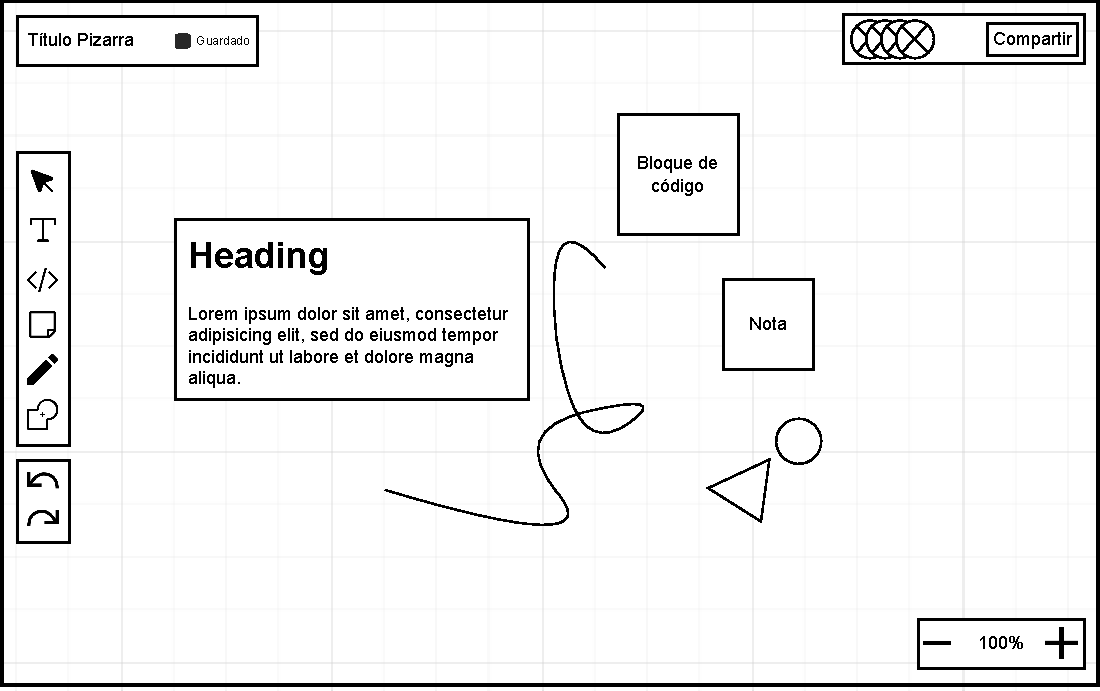
\includegraphics[width=\textwidth]{images/WireframePizarra.drawio.pdf}

Leyenda botones barra izquierda (arriba a abajo):
\begin{itemize}
    \item Botón de seleccionar.
    \item Insertar bloque de texto.
    \item Insertar bloque de código.
    \item Insertar nota.
    \item Dibujar.
    \item Insertar figura geométrica.
    \item Deshacer.
    \item Rehacer.
\end{itemize}

\textbf{\large Compartir pizarra:}\\[3mm]
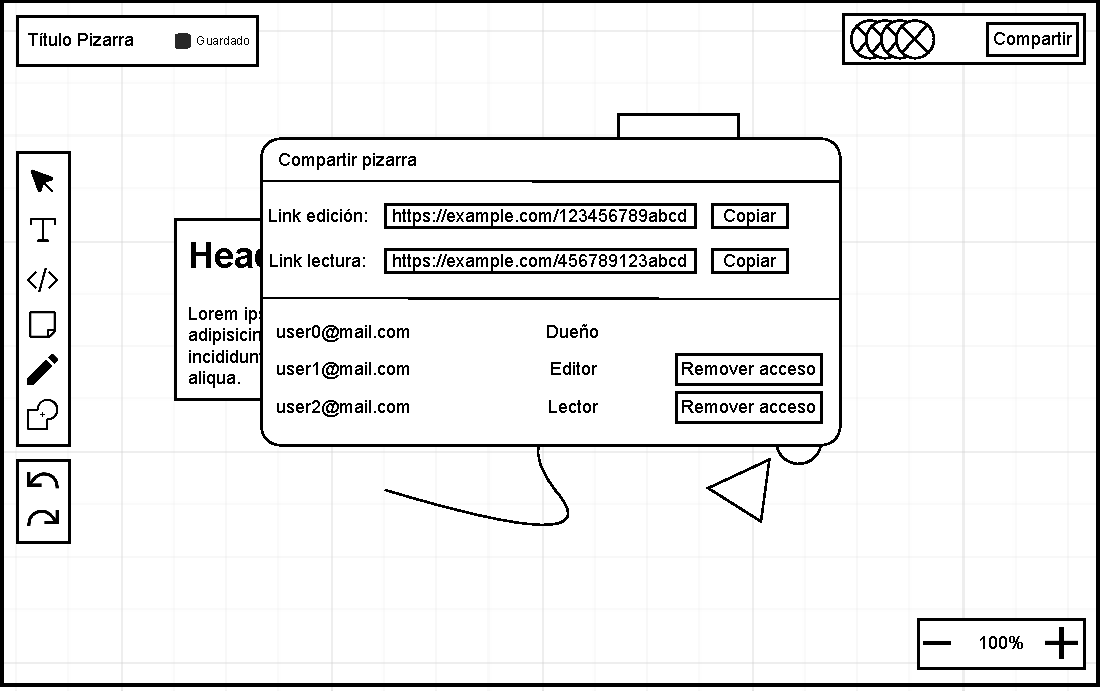
\includegraphics[width=\textwidth]{images/WireframePizarra-Ventana-compartir-pizarra.drawio.pdf}

\textbf{\large Lista de pizarras:}\\[3mm]
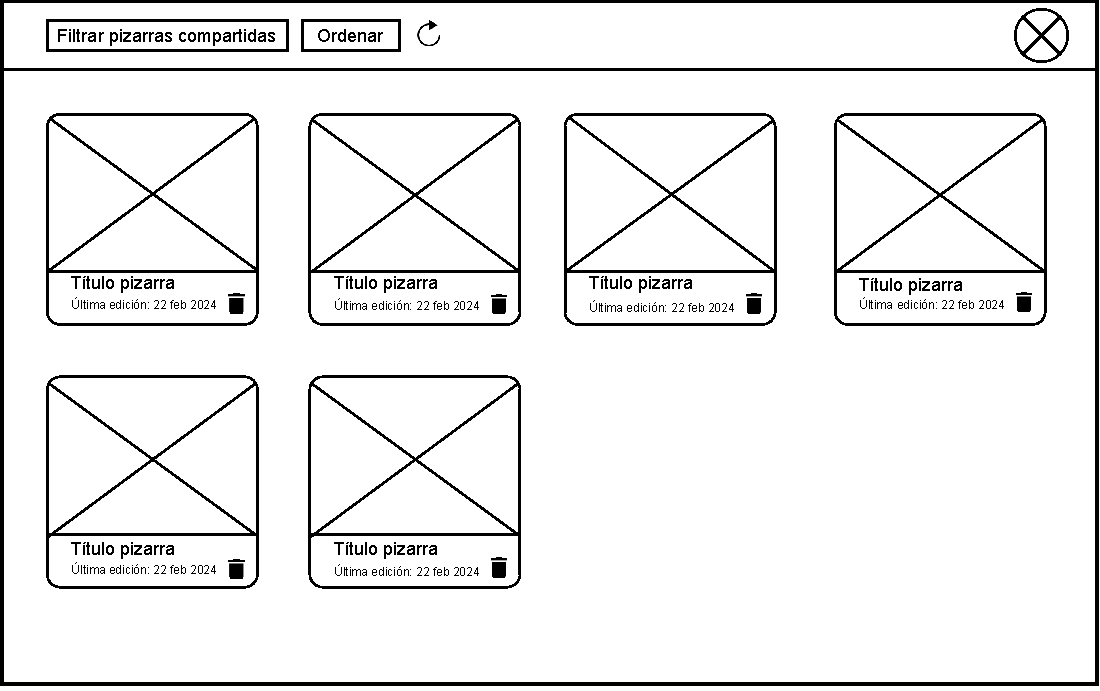
\includegraphics[width=\textwidth]{images/WireframeListaPizarras.drawio.pdf}

\end{document}
